\documentclass[11pt, a4paper]{article}

\usepackage[T1]{fontenc}
\usepackage{lmodern}
\usepackage[english]{babel}
\usepackage[utf8]{inputenc}
\usepackage{graphicx}
\usepackage{tikz}
\usepackage{amsmath}

\bibliographystyle{alpha}
\parindent 0pt

\begin{document}

\title{Evolutionary swarm robotics}
\author{Frank Lange\\Phillipp Schoppmann}
\date{June 28th 2013}
\maketitle
\thispagestyle{empty}

\begin{center}
\includegraphics[width = 0.6\textwidth]{pics/hulogo.pdf}
\end{center}

\vfill
\begin{abstract}\noindent
Evolutionary algorithms have proven to be useful optimization techniques in many different fields. This paper will describe the application of evolution to swarm robotics. It is based on research done by Dorigo et al. in 2004. \cite{swarmbots}
\end{abstract}

\newpage

\tableofcontents
\newpage


\section{Overview}
Swarm robotics focus on the coordination of multiple robots trying to reach a certain goal. In most scenarios, this involves limited communication abilities between robots and the restriction to local information. Although control is decentralized, as each robot is autonomous, emergent behavior can be observed, enabling the swarm to solve problems that a single robot can't.

\subsection{The Swarm Bot}
Here, the relevant artifact is called \emph{Swarm Bot}. It consists of several mobile \emph{S-Bots}, who can connect to and disconnect from each other.
\begin{figure}\centering
\includegraphics[width=0.8\textwidth]{pics/sbots2.jpg}
\caption{A swarm of six S-Bots, five of them connected}
\end{figure}
The Swarm Bot can be used for various tasks, including moving objects and moving through tough physical terrain. Furthermore, due to the ability to disconnect one or more S-Bots from itself, it can use them for tasks like finding a goal or tracing an optimal path, where single S-Bots may be more efficient.\\
In this paper we will focus on two tasks: \emph{Aggregation} and \emph{coordinated motion}. Aggregation describes the ability of several scattered S-Bots to minimize the distance between each other. Coordinated motion represents the ability of a connected Swarm Bot to move in a single direction. Both tasks are considered mandatory for the development of more complex behavior.

\subsection{Self organization}
As mentioned before, in most scenarios swarm robots are limited to local information. Therefore, it is important to apply mechanisms that can deal with this restriction while still being able to show emergent behavior.\\
\emph{Self organization} describes such mechanisms for biological systems, but can also be applied to swarm robotics. The System state depends on positive and negative feedback:\\
\emph{Positive feedback} represents the amplification of a certain property emerging from random interactions. It increases exponentially over time.\\
\emph{Negative feedback} works as a regulation which is triggered by positive feedback exhausting some resource. By the interaction of positive and negative feedback, the system is kept in a stable state. \cite[pp. 11--20]{camazine2003self}\\
The difficulty in creating self organizing Systems is the fact, that the relation between individual and global behavior is hard to analyze: Given a set of individual behaviors, it is difficult to predict the
behavior that is going to emerge on a system level. On the other hand, given global behavior, it is difficult to decompose individual behaviors leading to it.

\subsection{Artificial evolution}
A possible solution for this problem is \emph{artificial evolution}. It can be used to generate individual behavior, while evaluating the system as a whole and therefore bypassing the derivation of individual rules from global behavior. For the Swarm Bot, we will use artificial evolution to create controllers for each S-Bot. The controllers are realized through artificial neural networks, connecting sensory input to motor output. A genetic algorithm then determines optimal weight matrices for these networks.\\
Artificial evolution is based on the biological equivalent. It optimizes individuals on the basis of a given \emph{fitness function}, using \emph{selection}, \emph{reproduction} and \emph{mutation}. \cite[pp. 37--69]{eiben03genetic}\\
The general process of a genetic algorithm is as follows:
\begin{enumerate}
	\item An initial population is created randomly
	\item The fitness of all individuals in the current population is evaluated by applying the fitness function
	\item A subset of well-fit individuals is selected for reproduction
	\item Offspring is created and altered using mutation
	\item Steps 2--4 are repeated until a certain stop criterion (e.g. fitness threshold, timeout) is met
\end{enumerate}
Note that recombination is not used here, as it doesn't perform well for evolving weight matrices of neural networks. \cite[pp. 1425--1428]{yao1999evolving}


\subsection{Artificial neural networks}
As mentioned above, an artificial neural network is used to connect sensory input to motor output. Like genetic Algorithms, artificial neural networks are inspired by biology. There is a vast variety of different types of neural networks. Here, the relevant network architecture is the \emph{single layer perceptron}.

\begin{figure}\centering
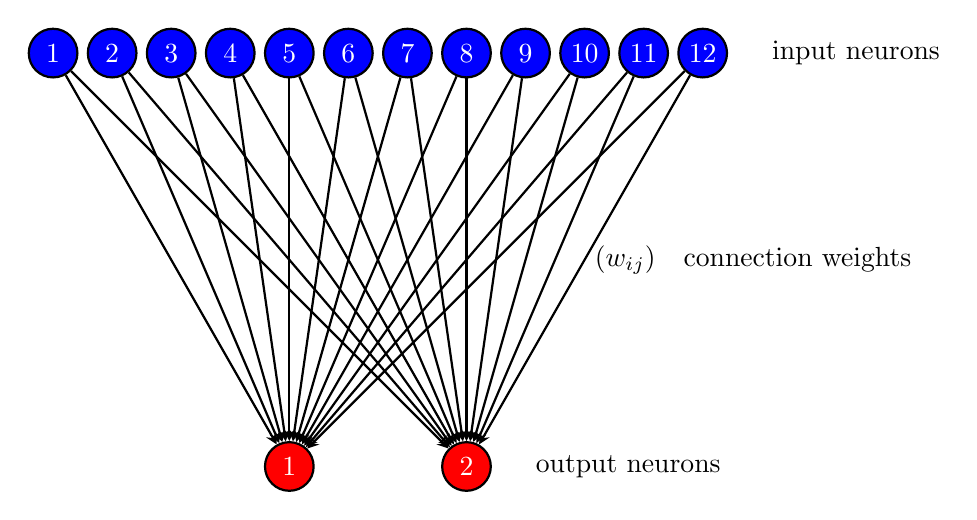
\begin{tikzpicture}[thick, scale=.75]
\node[circle, draw, fill=red, text=white] (O1) at (5, 0) {1};
\node[circle, draw, fill=red, text=white] (O2) at (8, 0) {2};
\foreach \i in {1, 2, ..., 12} {
	\node[circle, draw, fill=blue, label={center:\color{white}\i}] (I\i) at (\i, 7) {\phantom{0}};
	\draw[->, >=stealth] (I\i) -> (O1);
	\draw[->, >=stealth] (I\i) -> (O2);
}
\node[right] at (13,7) {input neurons};
\node[right] at (10, 3.5) {$\left( w_{ij} \right)$};
\node[right] at (11.5, 3.5) {connection weights};
\node[right] at (9,0) {output neurons};
\end{tikzpicture}
\caption{A single layer perceptron with 12 input neurons and two output neurons}
\end{figure}
The Neurons are arranged in two layers, one input and one output layer. Each input neuron is connected to each output neuron. All neural connections are \emph{weighted}.
A neuron's weighted input is mapped to its output using a given \emph{activation function}. Here, a \emph{sigmoid function} will be used:
\begin{figure}[h]\centering
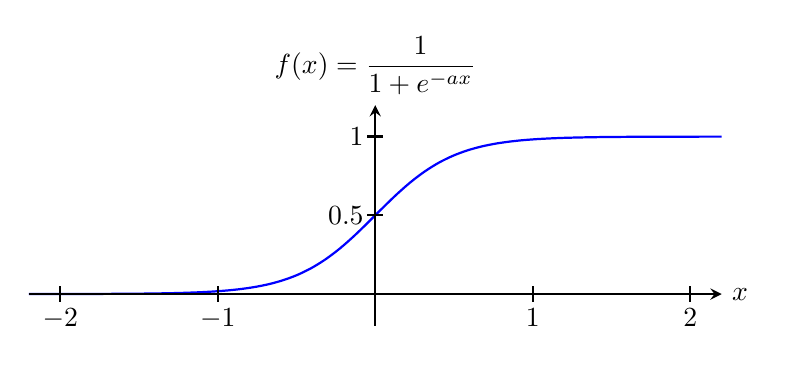
\begin{tikzpicture}[domain=-2.2:2.2, smooth, samples=50, >=stealth, scale=2, thick]

\draw[color=blue] plot (\x,{1 / (1+exp(- 4 *\x))}) node at (2.5, 0.7) {};

% Koordinatenachsen
\draw[->] (-2.2,0) -- (2.2,0) node[right] {$x$};
\draw[->] (0,-0.2) -- (0,1.2) node[above] {$f(x) = \dfrac{1}{1+e^{-ax}}$};
\draw (-0.05,1) --(0.05,1) node [left] {$1~$};
\draw (-0.05,0.5) -- (0.05,0.5) node [left] {$0.5~$};
\foreach \i in {-2, -1, 1, 2}{
	\draw (\i, -0.05) -- (\i, 0.05) node [below=1ex] {$\i$};
}
\end{tikzpicture}
\caption{The sigmoid function used in the experiment}\label{sigmoid}
\end{figure}
\newpage
The functionality of the network depends on the following parameters:
\begin{enumerate}
	\item Network topology, i.e. number of layers and neurons per layer
	\item The activation function
	\item Connection weights.
\end{enumerate}
In the following experiment, the S-Bot controllers only differ in (3).






%
% Experiments
%

\section{Experiment}
In the following section the experimental procedure is described. First we
introduce the general experimental environment and then continue to describe
the simulation details used in the aggregation and coordinated movement
experiments.

\subsection{Experimental setup}
As a general approach to the overall experiment a five step process was used
that can be roughly described as follows:

First the real robot hardware needs to be defined. After that a simulator is
developed that allows different detail levels for the agent models
representing the robots. Then a simplified model is used as a starting point
to construct experiments to evolve controllers for the S-Bots in a
reasonable amount of time. Successfully evolved controllers using the
simplified model are then improved using an increased level of detail.
Finally, the results of the experiments featuring the highest level of detail
are then ported to the real hardware.
\ \\
\begin{figure}[h]
  \centering
    \includegraphics[width=0.8\linewidth]{pics/01.jpg}
  \caption{a) Real hardware S-Bot b) Detailed simulation model c) Simplified
           simulation model}
  \label{}
\end{figure}

%
% Aggregation
%

\subsection{Aggregation}
For the aggregation experiments a very simplified model of the S-Bots was used.
Nearly every feature of the sbot was omitted, leaving only 2 wheels, 8
proximity sensors and 3 sound sensors.

\subsubsection{Simulation details}
The simulation environment consisted of a flat, obstacle free area covering an
equivalent of $3\times 3$ meters. In this area the S-Bots could move freely, permanently
emitting a sound signal that could be recognized within an approximate
radius of 75 cm. Noise was simulated by a uniformly distributed random signal
within 5\% of the senders saturation value.
\ \\

As described earlier a neural network was used to represent a successful
mapping of the data received by the 3 sound and 8 proximity sensors to the
motors of the 2 wheels of each S-Bot. Therefore the neural network consisted
of 12 input neurons (including a bias input) representing the input sensors
and which where each directly connected to the 2 output neurons representing
the motor outputs. Therefore the neural network contained 24 connections, with
each connection being weighted within [-10, +10] and represented by a 8-bit
bit string. This results in a $(12 \times 12) \times 8$ bit string representing a full
controller which is called the \textit{genotype}.

\subsubsection{Evolutionary algorithm}
The evolutionary algorithm starts with a random population of 100 genotypes,
each containing all the needed connection weights of the neural network and
therefore representing a full controller for the S-Bots.

These 100 random genotypes represent the first generation of an evolutionary
run, which in this experiment stretches over 100 generations.
To obtain a new generation of genotypes, each of the genotypes of the
current generation needs to be tested in the simulation environment described
above.
\ \\

To evaluate the aggregation performance of a single genotype, it is tested over
8 \textit{epochs} where the final performance value is the average of these
8 epochs. An epoch represents an experiment where a random number of S-Bots
between 4-8 is spawned in the simulation environment described above, each
configured with the current genotype to be tested. Each epoch lasts 900
simulation cycle and each simulation cycle represents 100 ms of real time.

The aggregation quality of a genotype for one epoch is measured by 2
performance criteria: how much did the S-Bots move to their center
of mass and how much did they move straight forward in doing so. Both criteria
are measured for each simulation cycle by averaging over the number of S-Bots
used in the specific epoch and are then multiplied. The final fitness of an
epoch is then achieved by averaging over the whole epoch duration. Again,
this is repeated 8 times for each of the 100 genotypes of the current
generation.
\ \\

After the evaluation of the entire generation the 20 best genotypes are then
selected to produce 5 offspring each. Mutation is applied by randomly flipping each bit with a
3\% chance.

After 100 generations the evolution stops, thus calling this an evolutionary
run. In the aggregation experiment 20 of those evolutionary runs where done
and the averaged performance of those 20 runs can be seen in Figure 2 where
it is important to keep in mind, that the performance is the product of both,
the gathering and the straight forward movement quality of the controllers.
\ \\

\begin{figure}[]
  \centering
    \includegraphics[width=0.6\linewidth]{pics/03.png}
  \caption{Aggregation performance averaged over 20 evolutionary runs}
  \label{}
\end{figure}

To evaluate the scalability of the evolved controllers each of those 20
controllers was then again tested against different group sizes in the pattern
4, 8, 12, \dots, 40 with 100 test runs for each group size. The final results of
that test can seen in Figure 3. This shows, that in theory, one can evolve
controller in an limited environment using only limited group sizes which
then still deliver acceptable performance once that is limit doesn't apply
anymore.However, it is worthy to keep in mind, that the simulation area of
$3\times 3$ meters was not scaled to cope with an increasing group size, hence
rendering it somewhat easy for larger groups to aggregate.
\ \\

\begin{figure}[h!]
  \centering
    \includegraphics[width=0.8\linewidth]{pics/06.png}
  \caption{Aggregation performance when confronted with increasing group sizes}
  \label{}
\end{figure}

\subsubsection{Observed behavior}
Completing the aggregation experiment are observed behaviors that seemed to
have been evolved in all evolutionary runs. These observations include that
solitary S-Bots seem to roam the complete area within large circles, whereas
smaller groups tend to develop a certain following behavior once aggregated,
where each S-Bot revolves around the center of the group and the group as a
whole moves around the area in small circles, always sticking together once
aggregated. Larger groups however never seem to reach a comparable stable
state. They slowly roam the area in larger circles, continuously picking up
but also losing single S-Bots.

%
% Coordinated Movement
%

\subsection{Coordinated Movement}
In the coordinated movement experiment the simplified simulation model was
used once more. However, the experiment is completely different compared to the
aggregation experiment, since now, it was tested whether controller could
be evolved that result in collective movement when a certain number of S-Bots
already are aggregated and physically connected.

\subsubsection{Simulation details}
In this experiment the same general simulation setup as within the aggregation
experiment was being used. Now however, the S-Bots are already connected via
rigid links representing their grippers. Therefore the sound and proximity
sensors from the aggregation experiment are being omitted and four
traction sensors are being introduced.

Hence the neural network now only features 5 input neurons, representing the
4 traction sensors and a bias neuron, being directly mapped to the 2 motor
output neurons. A connection weight is once again represented by a 8-bit
bit string mapping to the interval [-10, 10] but since there are less
connections in the neural network a single genotype only consists of $(5\times 2) \times 8$ bits.
\ \\

Since the rigid link between the S-Bots
does not prevent each S-Bot from having an orientation of it's own, the
traction sensors are connected to the links and are measuring the angle and
force of the traction received by each S-Bot. More precisely, via the
traction sensors each S-Bot receives the average direction and force in which
the group as a whole is trying to move and therefore can calculate the
difference between the average direction of the group and it's own orientation
and hence the severity of it's own misalignment compared to the majority of
the group.

\subsubsection{Evolutionary algorithm}
The evolutionary algorithm did not change significantly, compared to the
aggregation experiment. Once again it starts with 100 random genotypes as
a first generation and evolves each next generation by evaluating each
genotype for 5 epochs, where each epoch features a fixed group size of 4
S-Bots, including each S-Bot spawning with a different orientation. The
fitness of a controller is measured at the end of each epoch and is the
Euclidean distance between the group's starting position and the group's
position at the end of the epoch. The final fitness of a controller is again
the average of all 5 epochs, where each epoch consists of 150 simulation
cycles.
\ \\

One evolutionary run lasts 100 generation where in each generation the 20
best genotypes are selected to produce 5 offspring,
each with a 3\% chance of flipping each bit. After 20 evolutionary runs, the best genotype of each
run was selected and then tested again for increasing group sizes in the
pattern 4, 8, 12, ..., 40. The results are shown in Figure 4.

\begin{figure}[h]
  \centering
    \includegraphics[width=0.8\linewidth]{pics/15.png}
  \caption{Coordinated movement performance for increasing group sizes}
  \label{}
\end{figure}

\subsubsection{Observed behavior}
The behavior, that successful controllers seem to have evolved during the
evolutionary run seems to be, that the traction intensity determines how
drastically a single S-Bots changes it's orientation. This means that for
example if the S-Bots spawn with almost identical orientations, then the
traction received by each S-Bots is near 0 and so each can continue in that
exact direction with full speed. If however 3 S-Bots spawn with near identical
orientations and only one S-Bot spawns with a highly misaligned orientation,
then this S-Bot will receive an immense traction and will change it's
orientation drastically, whereas the other S-Bots will only tune their
orientation gracefully.
\ \\

This results in 2 side effects which are object avoidance and object pulling
behavior. When the group hits an object, the touching S-Bot receives the
impact as a high traction in the opposite direction to it's orientation and
the other S-Bots receive a similar traction and therefore change their
orientation rather drastically.
\ \\

Object pulling is possible with more evolved controllers where a certain
numbness has evolved in a positive fashion because it can be
beneficial for the group if a single S-Bot continues in it's own direction
even if it receives a slight traction in the opposite direction. Therefore,
if the S-Bots are connected to an object, the pulling S-Bots receive the
object as a slight traction in the opposite direction which to them is
identical to an S-Bot still trying to match the groups direction. Luckily
they ignore this traction hence resulting in them continuing their movement
and pulling the object as can be seen in Figure 5.
\ \\

\begin{figure}[h]
  \centering
    \includegraphics[width=0.65\linewidth]{pics/14.png}
  \caption{a) S-Bots connected to an object b) Resulting object pulling behavior}
  \label{}
\end{figure}


\section{Summary}
As we have learned, evolving controllers for a \emph{Swarm Bot} is possible, using a multi-stage approach. However, there are some drawbacks:\\
First, the evaluation of the fitness function requires global information. But in order to be able to adapt to new environments, S-Bots need to be able to evolve controllers during operation. With the current approach, only environments known at simulation time can be considered for evolution.\\
Second, the quality of evolved controllers depends on the quality of the simulation environment. As evolution on real hardware is unrealistic from a time perspective, the simulator has to implement as much detail as possible in order to evolve quality controllers. On the other hand, too much detail slows down the simulation significantly. Therefore, a good tradeoff between controller quality and simulation time has to be found.

\bibliography{references}

\end{document}
